\documentclass[landscape]{article}

% --- Page geometry: 48in x 36in landscape (standard Princeton conference poster) ---
\usepackage[paperwidth=48in, paperheight=36in, margin=1.3in, top=0in, bottom=0in, left=1.3in, right=1.3in, includeheadfoot=false]{geometry}

% --- Packages ---
\usepackage[T1]{fontenc}
\usepackage{mathpazo}
\usepackage{tgheros}      % TeX Gyre Heros — Helvetica/Roboto/Raleway-style sans-serif for title + headings
\usepackage{amsmath, amssymb}
\usepackage{multicol}
\usepackage{xcolor}
\usepackage{graphicx}
\usepackage{booktabs}
\usepackage{tabularx}
\usepackage{titlesec}
\usepackage{enumitem}
\usepackage{tikz}
\usetikzlibrary{shapes, arrows.meta, positioning, calc, backgrounds, shadings}
\usepackage{hyperref}

% --- Princeton orange (matched to princeton_logo.png background) ---
\definecolor{brandorange}{HTML}{D87B2D}
\definecolor{darkgray}{HTML}{333333}
\definecolor{lightcream}{HTML}{FBE9D6}

\hypersetup{colorlinks=true, urlcolor=brandorange, linkcolor=brandorange, citecolor=brandorange}

% --- Font sizes scaled up for poster viewing ---
\renewcommand{\normalsize}{\fontsize{25pt}{31pt}\selectfont}
\renewcommand{\small}{\fontsize{22pt}{27pt}\selectfont}
\renewcommand{\footnotesize}{\fontsize{20pt}{25pt}\selectfont}
\renewcommand{\large}{\fontsize{31pt}{37pt}\selectfont}
\renewcommand{\Large}{\fontsize{37pt}{43pt}\selectfont}
\renewcommand{\LARGE}{\fontsize{45pt}{51pt}\selectfont}
\renewcommand{\huge}{\fontsize{60pt}{68pt}\selectfont}
\renewcommand{\Huge}{\fontsize{84pt}{94pt}\selectfont}

% --- Section heading: centered bold sans-serif (Raleway-like) in brand orange + rule below ---
\titleformat{\section}[block]
  {\filcenter\color{brandorange}\sffamily\Large\bfseries}
  {}{0em}
  {}
  [{\color{brandorange}\titlerule[2pt]}]
\titlespacing*{\section}{0pt}{0.6em}{0.35em}

\titleformat{\subsection}[block]
  {\filcenter\color{brandorange}\sffamily\large\bfseries}
  {}{0em}
  {}
\titlespacing*{\subsection}{0pt}{0.5em}{0.25em}

\setlength{\parindent}{0pt}
\setlength{\parskip}{0.35em}
\setlength{\columnsep}{0.85in}
\setlength{\columnseprule}{0pt}

\pagestyle{empty}

\begin{document}

% =====================================================================
% TITLE BAR — flush to page edges (no margin), Princeton logo on right
% =====================================================================
\noindent\hspace*{-1.3in}%
\colorbox{brandorange}{%
\begin{minipage}[c][3.4in][c]{\dimexpr\paperwidth-2\fboxsep\relax}
\begin{minipage}[c]{0.20\paperwidth}\hfill\end{minipage}%
\begin{minipage}[c]{0.60\paperwidth}
\centering
\color{white}\sffamily
{\fontsize{76pt}{86pt}\selectfont \bfseries Spectral Filtering for Vision--Language--Action Models}\\[0.8em]
{\fontsize{28pt}{32pt}\selectfont Shivam Kak [sk3686@princeton.edu]\,$^{1}$ \quad
 Ishan Saha [is1893@princeton.edu]\,$^{1}$ \quad
 Connor Brown [cb6856@princeton.edu]\,$^{1}$}\\[0.35em]
{\fontsize{24pt}{28pt}\selectfont $^{1}$Princeton University}
\end{minipage}%
\begin{minipage}[c]{0.20\paperwidth}
\centering

\includegraphics[height=2.0in]{../../princeton_logo.png}
\end{minipage}%
\end{minipage}%
}

\vspace{1.5em}

% =====================================================================
% THREE-COLUMN BODY
% =====================================================================
\begin{multicols}{3}

% ---------------------------------------------------------------------
% COLUMN 1: motivation, background, four placements + diagram
% ---------------------------------------------------------------------
\section*{Abstract}

We integrate Spectral Transfer Units (STUs)~[2] into the $\pi_{0.5}$ flow-matching Vision--Language--Action model~[1] and evaluate them on LIBERO~[5] action prediction across \emph{four} architectural placements: post-hoc on the action expert; pre-input on the noisy action chunk; on the predicted velocity; and pre-input on the PaliGemma prefix. We compare against a parameter-matched diagonal-SSM (Mamba) control to isolate Hankel-specific structure. Across all placements, all spectral-filter counts $K$, all action horizons $H \in \{5,10,20,50\}$, and both warmup schedules, STU ties or underperforms the baseline. Mamba ties STU exactly, indicating the Hankel eigenbasis is not buying anything beyond generic linear recurrence in this regime. A short-warmup probe rules out the budget-bound hypothesis: forcing the spectral block to grow degrades the model. The result is a comprehensive negative finding that delineates where Hankel-eigenbasis filtering does and does not transfer.

\section*{Background: $\pi_{0.5}$ + Spectral Filtering}

\textbf{$\pi_{0.5}$ flow-matching VLA.} A SigLIP vision encoder + PaliGemma language model + a small action expert. An action chunk $a \in \mathbb{R}^{H \times D_a}$ is produced by integrating a learned velocity field
$$x_{t+\mathrm{d}t} = x_t + \mathrm{d}t \cdot v_\theta(x_t, t), \quad x_0 \sim \mathcal{N}(0, I).$$
The action expert sees the full chunk in parallel, so causal attention is the only mechanism mixing information across the $H$ time positions of the chunk---a natural fit for spectral methods.

\textbf{Spectral Transfer Units (STU).} Convolve along the horizon with eigenvectors $\phi_k$ of the Hankel matrix $Z_{ij} = \frac{2}{(i+j)^3 - (i+j)}$, scaled by the fourth root of their eigenvalues:
$$y = \sum_{k=1}^{K} \!\Bigl( (u * \phi_k^+)\, M_k^+ \,+\, (u * \phi_k^-)\, M_k^- \Bigr)$$
where $\phi_k^\pm$ split filters into even/odd-symmetric components, $M_k^\pm$ are learnable, FFT in $O(L \log L)$.

\textbf{Mamba-style control.} Parameter-matched diagonal SSM $\dot x = Ax + Bu,\, y = Cx$ with HiPPO-LegS init. Isolates whether \emph{Hankel-specific} structure helps vs.\ generic linear recurrence (per midterm reviewer ask).

\section*{Architectural Placements}

\textbf{v1 (post-hoc, action expert):} residual STU \emph{after} the action-expert transformer, randomly initialized.\\[-0.3em]
\textbf{v2 (pre-input, action expert):} STU on the noisy action chunk $x_t$ \emph{before} the transformer; zero-init out-projection so step~0 is bit-identical to baseline.\\[-0.3em]
\textbf{v3 (output velocity):} STU on predicted $v_t \in \mathbb{R}^{B \times H \times 32}$, the natural axis for a ``smoothness'' prior.\\[-0.3em]
\textbf{v4 (PaliGemma prefix):} mirror of v2 on the VLM side; STU on the prefix embeddings ($\sim$968 image+language tokens) before the VLM forward, zero-init out-projection.

\vspace{0.6em}
\begin{center}
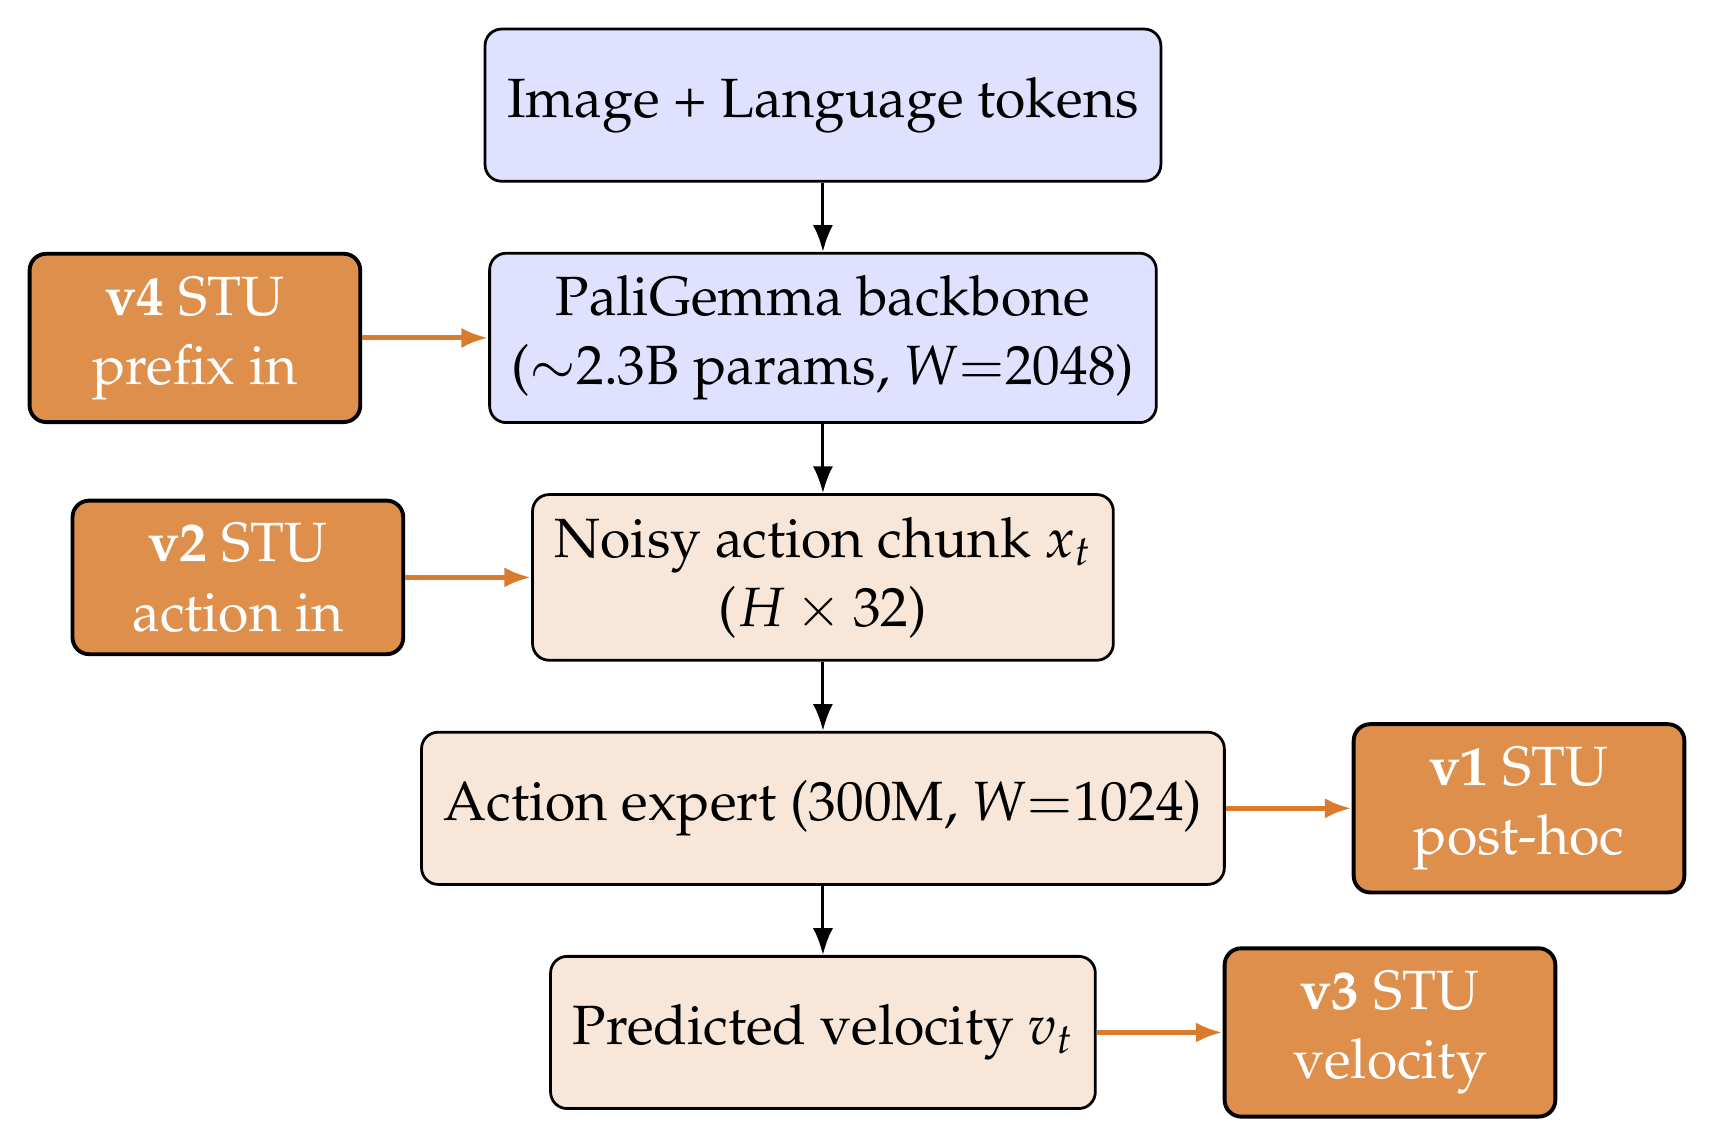
\begin{tikzpicture}[
    node distance=1.0em,
    box/.style={draw, rounded corners=6pt, align=center, minimum height=2.2em, font=\footnotesize, inner sep=8pt, line width=1.0pt},
    vlm/.style={box, fill=blue!12, minimum width=6.6cm},
    act/.style={box, fill=brandorange!18, minimum width=6.6cm},
    stuv/.style={box, fill=brandorange!85, text=white, line width=1.4pt, minimum width=4.2cm},
    arrow/.style={-{Latex[length=3.4mm]}, line width=1.1pt},
    redarrow/.style={-{Latex[length=3.4mm]}, line width=1.8pt, brandorange},
]
% Main path
\node[vlm] (img) {Image + Language tokens};
\node[vlm, below=of img] (palig) {PaliGemma backbone\\\footnotesize($\sim$2.3B params, $W{=}2048$)};
\node[act, below=of palig] (chunk) {Noisy action chunk $x_t$\\\footnotesize($H \times 32$)};
\node[act, below=of chunk] (expert) {Action expert (300M, $W{=}1024$)};
\node[act, below=of expert] (vel) {Predicted velocity $v_t$};
\draw[arrow] (img) -- (palig);
\draw[arrow] (palig) -- (chunk);
\draw[arrow] (chunk) -- (expert);
\draw[arrow] (expert) -- (vel);
% v4 (left of palig)
\node[stuv, left=1.6cm of palig] (v4) {\textbf{v4} STU\\prefix in};
\draw[redarrow] (v4.east) -- (palig.west);
% v2 (left of expert input)
\node[stuv, left=1.6cm of chunk] (v2) {\textbf{v2} STU\\action in};
\draw[redarrow] (v2.east) -- (chunk.west);
% v1 (right of expert)
\node[stuv, right=1.6cm of expert] (v1) {\textbf{v1} STU\\post-hoc};
\draw[redarrow] (expert.east) -- (v1.west);
% v3 (right of vel)
\node[stuv, right=1.6cm of vel] (v3) {\textbf{v3} STU\\velocity};
\draw[redarrow] (vel.east) -- (v3.west);
\end{tikzpicture}
\end{center}
\textbf{Figure 1.} The four sites in $\pi_{0.5}$ where we tested an STU residual block. v1 is the original midterm design; v2/v3/v4 share the dreamer-aligned recipe (pre-input or pre-output, zero-init out-projection). Each placement isolates a different question: whether residual STUs help \emph{after} a converged action expert (v1), at the chunk-input or velocity-output stages where horizon mixing is most plausible (v2/v3), or on the much larger vision-language backbone where capacity may be less of a bottleneck (v4).

% ---------------------------------------------------------------------
% COLUMN 2: experimental setup, results, figures, tables
% ---------------------------------------------------------------------
\columnbreak

\section*{Experimental Setup}

\textbf{Training.} Fine-tune from $\pi_{0.5}$ \emph{base} (\texttt{gs://openpi-assets/checkpoints/pi05\_base})---\emph{not} the LIBERO-finetuned checkpoint. AdamW $5{\times}10^{-5}$, cosine decay (10k or 1k warmup), batch 8, gradient clip 1.0, bfloat16, 5000 steps per run.

\textbf{Compute.} \textbf{26 LIBERO fine-tunes}, $\sim$30 GPU-hours on Princeton's \texttt{della} cluster (H100 NVL 95\,GB and 2$\times$\,RTX PRO 6000 Blackwell 97\,GB).

\textbf{Evaluation.} Last-100-step mean training loss (smoothed flow-matching MSE) is the reported metric; differences below $\pm 1\%$ are within run-to-run noise.

\section*{Results: $H{=}10$ Architecture Comparison}

\begin{minipage}{\linewidth}
\centering
\footnotesize
\begin{tabular}{@{}lccc@{}}
\toprule
\textbf{Model} & \textbf{Final Loss} & \textbf{$\Delta$ Base} & \textbf{Params} \\
\midrule
Baseline                       & \textbf{0.0299} & ---     & 0 \\
STU-K4 (post-hoc)              & 0.0316 & $+5.7\%$ & 8.4M  \\
STU-K8 (post-hoc)              & 0.0313 & $+4.7\%$ & 16.8M \\
Mamba-K4 (post-hoc)            & 0.0311 & $+4.0\%$ & 8.4M  \\
Mamba-K8 (post-hoc)            & 0.0312 & $+4.3\%$ & 16.8M \\
\midrule
\textbf{STU-v2-K4 (act-input)}    & \textbf{0.0298} & $\mathbf{-0.5\%}$ & 8.4M  \\
\textbf{STU-v2-K8 (act-input)}    & \textbf{0.0298} & $\mathbf{-0.4\%}$ & 16.8M \\
\textbf{STU-v3-K4 (output vel)}   & \textbf{0.0297} & $\mathbf{-0.6\%}$ & 0.07M \\
\textbf{STU-v4-K4 (PaliGemma)}    & \textbf{0.0296} & $\mathbf{-1.2\%}$ & 33.6M \\
\textbf{STU-v4-K8 (PaliGemma)}    & \textbf{0.0296} & $\mathbf{-1.0\%}$ & 67.1M \\
\bottomrule
\end{tabular}
\\[0.4em]
\raggedright
\textbf{Table 1.} Last-100-step mean loss at $H{=}10$. Post-hoc residuals \emph{hurt}; all three zero-init pre-input placements (v2, v3, v4) recover baseline within run-to-run noise.
\end{minipage}

\begin{center}
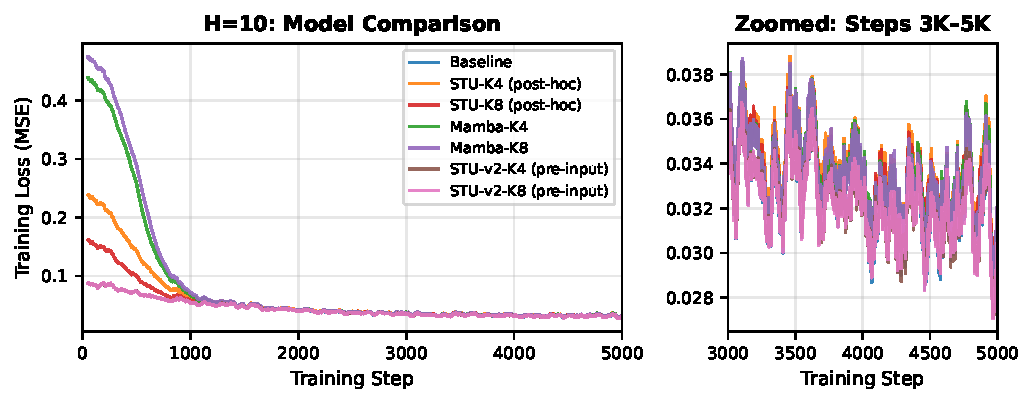
\includegraphics[width=\linewidth]{h10_comparison.pdf}
\end{center}
\textbf{Figure 2.} $H{=}10$ training loss (50-step rolling mean). Post-hoc variants (orange/green) start with elevated loss and only catch up by step $\sim$2000. Zero-init STU-v2 (brown) overlaps baseline (blue) from step 0---the visual signature of zero-init.

\section*{Horizon Ablation}

\begin{center}
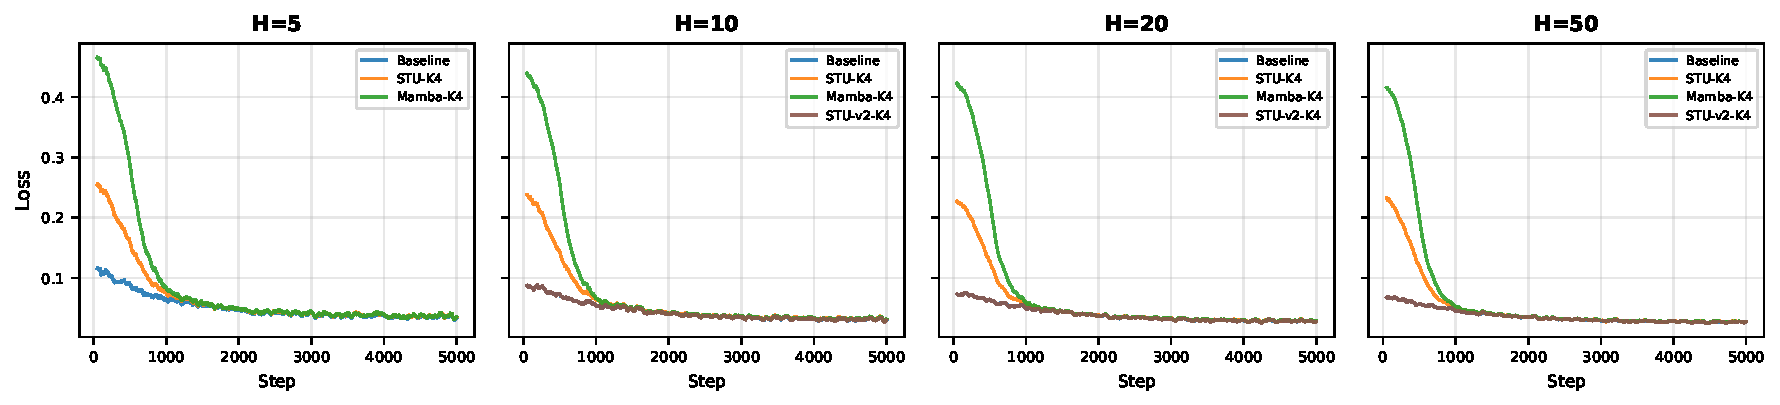
\includegraphics[width=\linewidth]{horizon_ablation.pdf}
\end{center}
\textbf{Figure 3.} Horizon sweep ($H \in \{5, 10, 20, 50\}$). Post-hoc variants elevated at every horizon. STU-v2 (brown) overlaps baseline from step 0 at every horizon. Longer $H$ reaches lower terminal MSE because each loss value averages more correlated time-steps.

\begin{minipage}{\linewidth}
\centering
\footnotesize
\begin{tabular}{@{}lcccc@{}}
\toprule
\textbf{$H$} & \textbf{Base} & \textbf{STU-K4 post-hoc} & \textbf{STU-v2-K4} & \textbf{STU-v4-K4} \\
\midrule
5  & 0.0338 & 0.0352 ($+4.2\%$) & --- & --- \\
10 & 0.0299 & 0.0316 ($+5.7\%$) & \textbf{0.0298} & \textbf{0.0296} \\
20 & 0.0276 & 0.0286 ($+3.5\%$) & \textbf{0.0275} & \textbf{0.0275} \\
50 & 0.0269 & 0.0274 ($+1.9\%$) & \textbf{0.0270} & --- \\
\bottomrule
\end{tabular}
\\[0.4em]
\raggedright
\textbf{Table 2.} Horizon ablation, all warmup-10k. Post-hoc gap shrinks ($+5.7\%$ @ 10 $\to +1.9\%$ @ 50) but does not close. Linear extrapolation crosses zero only at $H \approx 80$--100, beyond LIBERO. Zero-init v2 \& v4 tie baseline at every horizon tested.
\end{minipage}

\section*{Spectral Weight Analysis}

We loaded the v2 checkpoints and inspected $M_k^\pm$ directly to verify the spectral block is being trained:
$$\max|M^\pm_k| \approx 8\!\times\!10^{-3}, \quad \overline{|M^\pm_k|} \approx 7\!\times\!10^{-4}$$
Frobenius norms 0.29--0.49 across the full $K \times D_a \times W$ tensor. Default random-init scale would be $(KD_a)^{-1/2} \approx 0.088$, so after 5k steps $M_k^\pm$ has grown to about \textbf{1\% of a typical layer's magnitude}. The optimizer has measurably moved $M_k^\pm$ off zero, but not enough to materially alter the network's output.

% ---------------------------------------------------------------------
% COLUMN 3: warmup probe, key findings, discussion, future work
% ---------------------------------------------------------------------
\columnbreak

\section*{Warmup Schedule Sensitivity}

Shortening LR warmup from 10k to 1k steps causes $\|M^+\|_F$ to grow from 0.36 to 0.92 ($2.5\times$), forcing the spectral block off zero-init faster.

\begin{minipage}{\linewidth}
\centering
\footnotesize
\begin{tabular}{@{}lcccc@{}}
\toprule
& \textbf{Base} & \textbf{v2-K4} & \textbf{v3-K4} & \textbf{v4-K4} \\
\midrule
warmup-10k & 0.0299 & $-0.5\%$ & $-0.6\%$ & $-1.2\%$ \\
warmup-1k  & 0.0277 & $+1.5\%$ & $+2.0\%$ & $+1.9\%$ \\
\bottomrule
\end{tabular}
\\[0.4em]
\raggedright
\textbf{Table 3.} Warmup probe at $H{=}10$, all three zero-init placements. Absolute loss improves with shorter warmup at every site, but the relative position of every STU variant \emph{worsens} when $M_k^\pm$ is allowed to grow---consistent across all three placements. \textbf{This rules out the budget-bound explanation:} more learning signal $\to$ \emph{worse}, not better.
\end{minipage}

\section*{Key Findings}

\colorbox{lightcream}{\parbox{\dimexpr\linewidth-2\fboxsep\relax}{%
\begin{enumerate}[leftmargin=1.6em, nosep, label=\textbf{\arabic*.}]
\item \textbf{Negative result is robust across 4 placements} (post-hoc, action-input, output-velocity, VLM-prefix), all $K$, all $H$, both warmups. Spectral filtering does not add a useful inductive bias for $\pi_{0.5}$ action prediction on LIBERO.
\item \textbf{Hankel structure is irrelevant here.} Mamba ties STU at every configuration tested, so the Hankel eigenbasis is not buying anything beyond generic linear recurrence.
\item \textbf{The horizon hypothesis is directionally right but quantitatively weak.} The post-hoc gap shrinks with $H$, but linear extrapolation crosses zero only at $H \approx 80$--$100$, beyond LIBERO.
\item \textbf{Placement and zero-init matter more than the spectral basis.} The pre-input zero-init recipe rescues the negative result everywhere (no longer hurts), but never produces a positive one.
\item \textbf{Even on the much larger PaliGemma backbone (v4),} with $25\times$ more parameters than the action expert, the result is unchanged. The headroom hypothesis is not the explanation.
\end{enumerate}
}}

\section*{Discussion}

\textbf{Why doesn't the spectral block engage?} The dreamer-aligned recipe makes the residual branch start at zero, but it does not give it any reason to leave zero. With $H{=}10$ noisy chunks predicted from a near-converged backbone, the per-step MSE gradient already lives in the action expert's existing weight space; the optimizer has no incentive to route it through a freshly-initialised parallel pathway. The 1k-warmup probe makes this concrete: when we force $M_k^\pm$ to grow $2.5\times$, performance \emph{worsens} at every placement.

\textbf{The horizon hypothesis is real but small.} The post-hoc gap shrinks monotonically from $+5.7\%$ at $H{=}10$ to $+1.9\%$ at $H{=}50$, validating the directional claim from our midterm. But linear extrapolation crosses zero only at $H \approx 80$--$100$, well beyond what LIBERO action chunks support. The spectral inductive bias has the right shape; the wrong magnitude.

\textbf{Architecture matters, structure does not.} Mamba-K\{4,8\} ties STU at every configuration, so the cost---and the benefit---of inserting a new linear-recurrence branch is dominated by \emph{where} you put it and \emph{how} you initialise it, not by the choice of Hankel eigenbasis vs.\ HiPPO-LegS diagonal SSM.

\section*{Future Work}

\begin{itemize}[leftmargin=1.4em, nosep]
\item Success rates on the 130 LIBERO tasks (we measure only training MSE; rollout behavior could differ even at near-equal MSE).
\item A generic-SSM control on the VLM side (Mamba-v4): the FFT-based diagonal-SSM kernel exceeds 32~GB on the 968-position prefix at $W{=}2048$; a chunked-FFT or selective-scan re-implementation would close this gap.
\item STU-v3 at $H \in \{20, 50\}$ and STU-v4 at $H{=}50$ (compute-bound).
\item A learned residual gate, to verify the optimizer is not actively zeroing the block.
\item Pre-training a $\pi_{0.5}$ checkpoint \emph{from scratch} with the spectral block in place, to test whether STU helps when not introduced as a residual on a converged backbone.
\end{itemize}

\section*{References}
{\footnotesize
\begin{enumerate}[leftmargin=1.4em, nosep, label={[\arabic*]}]
\item Physical Intelligence. $\pi_0$: A Vision-Language-Action Flow Model. \textit{arXiv:2410.24164}, 2024.
\item Agarwal, N., Hazan, E., et al. Spectral State Space Models. \textit{arXiv:2312.06837}, 2023.
\item Gu, A., Dao, T., Ermon, S., Rudra, A., R\'e, C. HiPPO: Recurrent Memory with Optimal Polynomial Projections. \textit{NeurIPS}, 2020.
\item Gu, A., Dao, T. Mamba: Linear-Time Sequence Modeling with Selective State Spaces. \textit{arXiv:2312.00752}, 2023.
\item Liu, B., et al. LIBERO: Benchmarking Knowledge Transfer for Lifelong Robot Learning. \textit{NeurIPS}, 2023.
\item Physical Intelligence. OpenPI. \url{https://github.com/Physical-Intelligence/openpi}, 2024.
\end{enumerate}
}

\section*{Acknowledgements}

We thank Professor Dhruv Shah, instructor of ECE~534, and teaching assistants Lihan Zha and Asher Hancock for their feedback that informed the direction of this project. Compute provided by the Princeton \texttt{della} cluster.

\end{multicols}

% =====================================================================
% FOOTER BAR — flush to page edges (no margin)
% =====================================================================
\vfill
\noindent\hspace*{-1.3in}%
\colorbox{brandorange}{%
\begin{minipage}[c][1.0in][c]{\dimexpr\paperwidth-2\fboxsep\relax}
\color{white}\sffamily
\hspace*{1.5in}{\Large \href{https://github.com/ishansaha01/vla-stu}{\color{white}\texttt{https://github.com/ishansaha01/vla-stu}}} \hfill
{\Large \bfseries ECE 534} \hfill
{\Large \texttt{sk3686, is1893, cb6856 @princeton.edu}}\hspace*{1.5in}
\end{minipage}%
}

\end{document}
